
\begin{table}
 \begin{tabular}{p{100pt}|p{230pt}}
  \hline\hline
   name & value ranges \\
  \hline
   \mbox{(a) no VSE} \break \phantom{(a)} 18 elements &
       [0, 1, 2, 3, 4, 5, 6, 7, 8, 9, 10, 11, 12, 13, 14, 15, 16, 17] \\ \hline
   \mbox{(b) 2-VSE} \break  \phantom{(a)} $11 + 10$ elements &
     \mbox{[0, 1, 2, 3, 4, 5, 6, 7, 8, 9, L]}\break + [0, S, 10, 11, 12, 13, 14, 15, 16, 17] \\ \hline
   \mbox{(c) 3-VSE} \break \phantom{(a)} $9 {+} 9 {+} 6$ elements &
     \mbox{[0, 1, 2, 3, 4, 5, 6, 7, L] + [0, S, 8, 9, 10, 11, 12, 13, L]}\break + [0, S, 14, 15, 16, 17] \\ \hline
   \mbox{(d) 4-VSE} \break \phantom{(a)} $7 {+} 7 {+} 7 {+} 6$ elements &
     \mbox{[0, 1, 2, 3, 4, 5, L] + [0, S, 6, 7, 8, 9, L]}\break + [0, S, 10, 11, 12, 13, L] + [0, S, 14, 15, 16, 17] \\ \hline
 \end{tabular}
\end{table}

\begin{table}
 \begin{tabular}{|C{15pt}|C{15pt}|C{15pt}|C{15pt}|C{15pt}|C{15pt}|C{15pt}|C{15pt}|C{15pt}|C{15pt}|C{15pt}|C{15pt}|C{15pt}|C{15pt}|C{15pt}|C{15pt}|C{15pt}|C{15pt}|}
  \multicolumn{18}{l}{(a) 1 layer with 18 elements}\\\hline
   0 & 1 & 2 & 3 & 4 & 5 & 6 & 7 & 8 & 9 & 10 & 11 & 12 & 13 & 14 & 15 & 16 & 17 \\\hline
  \multicolumn{18}{l}{}\\
  \multicolumn{18}{l}{(b) 2 layers with $11 + 10$ elements}\\\hline
   0 & 1 & 2 & 3 & 4 & 5 & 6 & 7 & 8 & 9 & \multicolumn{8}{c|}{L ($10 \le x$)} \\\hline
   0 & \multicolumn{9}{c|}{S ($1 \le x \le 9$)} & 10 & 11 & 12 & 13 & 14 & 15 & 16 & 17 \\\hline
  \multicolumn{18}{l}{}\\
  \multicolumn{18}{l}{(b) 3 layers with $9 + 9 + 6$ elements}\\\hline
   0 & 1 & 2 & 3 & 4 & 5 & 6 & 7 & \multicolumn{10}{c|}{L ($8 \le x$)} \\\hline
   0 & \multicolumn{7}{c|}{S ($1 \le x \le 7$)} & 8 & 9 & 10 & 11 & 12 & 13 & \multicolumn{4}{c|}{L ($14 \le x$)}\\\hline
   0 & \multicolumn{13}{c|}{S ($1 \le x \le 13$)} & 14 & 15 & 16 & 17 \\\hline
  \multicolumn{18}{l}{}\\
  \multicolumn{18}{l}{(b) 4 layers with $7 + 7 + 7 + 6$ elements}\\\hline
   0 & 1 & 2 & 3 & 4 & 5 & \multicolumn{12}{c|}{L ($6 \le x$)} \\\hline
   0 & \multicolumn{5}{c|}{S ($1 \le x \le 5$)} & 6 & 7 & 8 & 9 & \multicolumn{8}{c|}{L ($10 \le x$)}\\\hline
   0 & \multicolumn{9}{c|}{S ($1 \le x \le 9$)} & 10 & 11 & 12 & 13 & \multicolumn{4}{c|}{L ($14 \le x$)}\\\hline
   0 & \multicolumn{13}{c|}{S ($1 \le x \le 13$)} & 14 & 15 & 16 & 17 \\\hline
 \end{tabular}
\end{table}

\begin{table}
\centering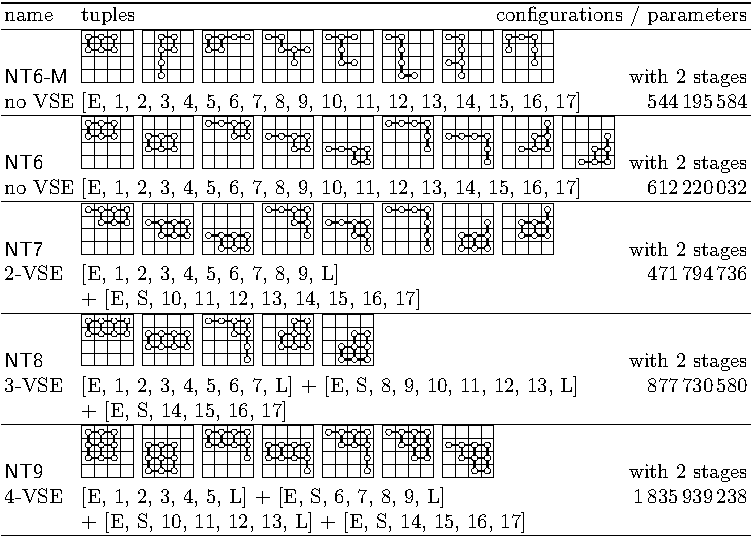
\includegraphics[]{figures/NT-table.pdf}
\end{table}

% 6G      NUM_TUPLES=8 NUM_SPLIT=1 で積は 48  メモリは  4.9GB (18^6*8*1*2*4*4)
% 6タプル NUM_TUPLES=9 NUM_SPLIT=1 で積は 54  メモリは  4.9GB (18^6*9*1*2*4*4)
% 7タプル NUM_TUPLES=7 NUM_SPLIT=2 で積は 98  メモリは  8.8GB (11^7*7*2*2*4*4)
% 8タプル NUM_TUPLES=5 NUM_SPLIT=3 で積は 120 メモリは 20.7GB ( 9^8*5*3*2*4*4)
% 9タプル NUM_TUPLES=7 NUM_SPLIT=4 で積は 252 メモリは 36.2GB ( 7^9*7*4*2*4*4)
